\documentclass{article}

% Import necessary packages.
\usepackage{amsmath}
\usepackage{graphicx}
\usepackage{media9}
\usepackage{algpseudocode}
\usepackage{algorithm}
\usepackage{caption}
\usepackage{amsthm}
\usepackage{thmtools}
\usepackage{subcaption}
\usepackage{tikz}
\usepackage{xcolor}
\usepackage{amsfonts}
\usepackage{transparent}
\usepackage{hyperref}
\usepackage{xcolor}
\usepackage{framed}
\usepackage{adjustbox}
\usepackage{multimedia}
\usepackage{tcolorbox}
\usepackage{float}
\usepackage{geometry}

\newtheorem{theorem}{Theorem}
\newtheorem{lemma}{Lemma}
\newtheorem{corollary}{Corollary}
\newtheorem{definition}{Definition}

\theoremstyle{definition}
\newtheorem{example}{Example}

\theoremstyle{remark}
\newtheorem*{remark}{Remark}

\title{Intersecting lines in 2 dimensions}

\begin{document}

\maketitle

{\bf Keywords}
\begin{itemize}
    \item Gilbert model
    \item Planar graphs
    \item Road networks
    \item (Voronoi lattice)
\end{itemize}

\section{The model}
We are going to generate networks with underlaying geometric constraint. Procedure to generate a network of size $n$ is as follows:
\begin{enumerate}
    \item Initialize the unit hypercube $[0,1]^2$.
    \item Pick a point $P\in (0,1)^n$ uniformly at random.
    \item Pick a direction vector $v\in \mathbb{R}^n$ uniformly at random.
    \item For the line given by the beginning point and extension in both the $v$ as well as the $-v$ direction.
    \item Determine the closest intersection points $Q_1$, $Q_2$ on both sides. This is either with an already existing line or with the boundary of the unit hypercube.
    \item Add the resulting line segment to the unit hypercube.
    \item Repeat this procedure $n$ times.
    \item Form a network by representing every line as a vertex and adding an edge between two lines whenever they intersect.
\end{enumerate}

\begin{figure}
    \centering
    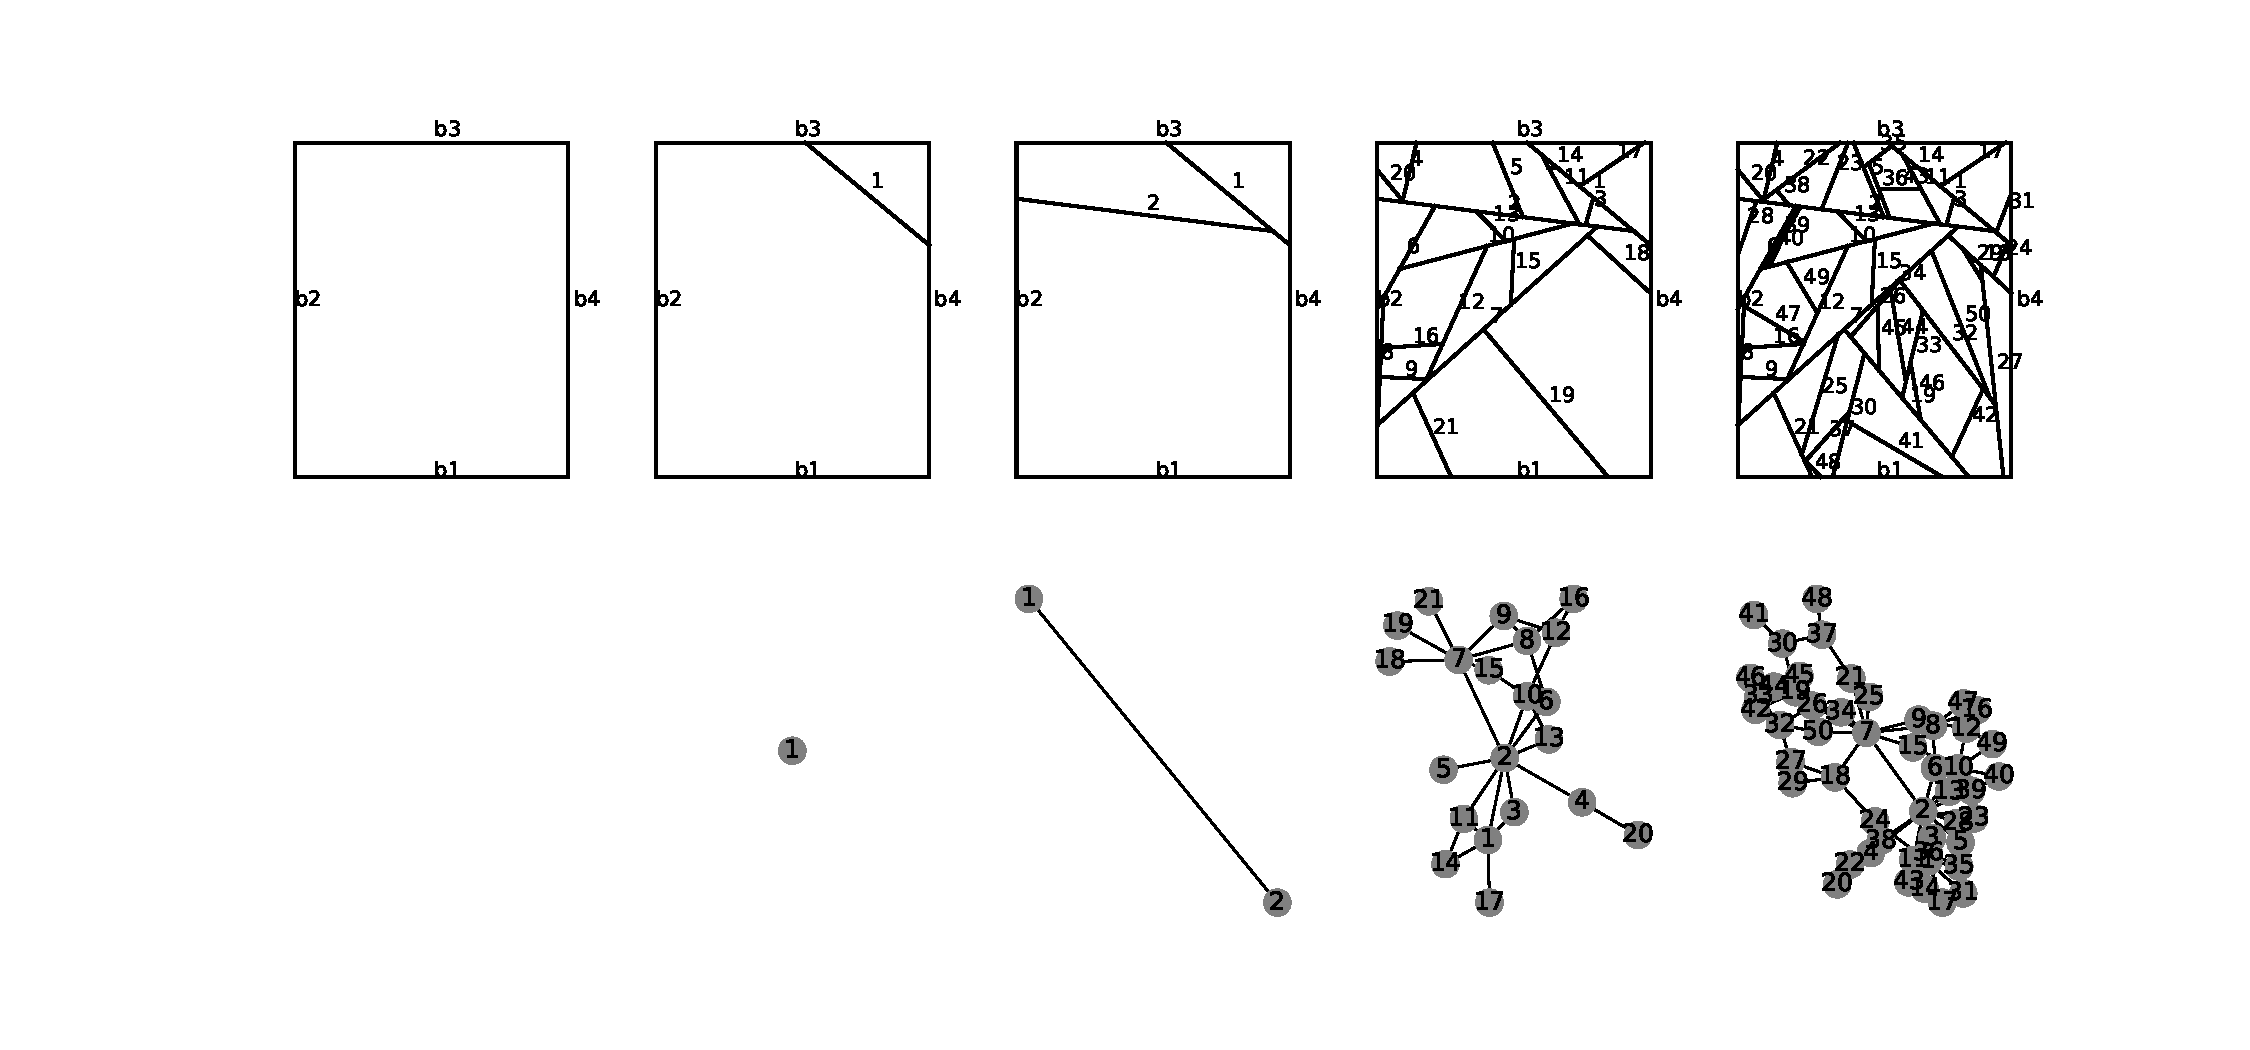
\includegraphics[width=\linewidth]{Figures/NetworkEvolution.pdf}
    \caption{Example of a network generated with the above procedure.}
    \label{fig:Example}
\end{figure}

\section{Results}

\begin{lemma}
    Every random direction graph (RDG) is planar. 
\end{lemma}
\begin{proof}
    We know a graph is planar whenever it does not contain the complete graph $K_6$ or the complete bipartite graph $K_{3,3}$ as a minor~(Wagner's theorem). We will check for both instances that this situation can not occur under RDG graph generation.

    $\mathbf{K_{6}}$ \\
    To show that $K_6$ can not occur we will try to construct a corresponding sequence of line segments. Note that since we work with straight lines we can never have a clique of size larger than three. Therefore, $K_6$ can not occur. We provide a visual interpretation nevertheless.
    \begin{figure}[h!]
        \centering
        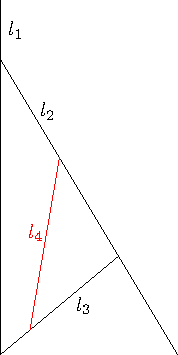
\includegraphics{Figures/K6}
        
        \caption{Note that $K_6$ can never occur because we are working with straight lines.}\label{fig:Planar_Proof_K6}
    \end{figure}

    $\mathbf{K_{3,3}}$ \\
    In the case of $K_{3,3}$ we can do the same thing. We incrementally add lines, starting with vertex $v_1$. Note that because of symmetry the starting vertex does not matter. In Figure~\ref{fig:Planar_Proof_K33} we see that $K_{3,3}$ can never be constructed.

    \begin{figure}
        \centering
        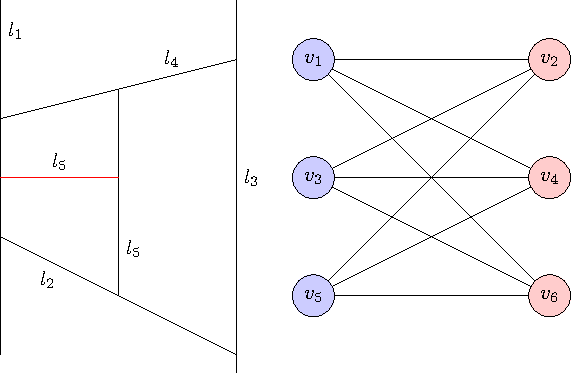
\includegraphics{Figures/K33.pdf}
        \caption{$K_{3,3}$}
        \label{fig:Planar_Proof_K33}
    \end{figure}
    
\end{proof}

\begin{lemma}
    In the limit of the network size ($n$) going to infinity, the average degree of a RDG realization is given by:
    \begin{align}
        \lim_{n \to \infty} \langle k \rangle_{n} := \lim_{n \to \infty} \frac{1}{n} \sum_{i=1}^{n} d_i = 4.
    \end{align}
\end{lemma}
\begin{proof}
    Probability of hitting the border goes to zero (+mathematical details).
\end{proof}


Note that
\begin{align}
    P_{k_i\mapsto k_i+1}(l_i) &= \sum_{j \in N(\sum_{i}A_i)} \int_{A_j} \mathbb{P}\{ \text{hitting } l+i \ | \ X=x \} d\lambda, \label{eq:general} \\
    \text{where } N \left(\sum_{i}A_i \right) :&= \bigg\{ j \in [t] \ s.t. \ A_j \text{ is adjacenct to } A_i \bigg\}
\end{align}

For square networks where we sample direction vector $v \in S^{1}$, we know that:
\begin{align}
    \mathbb{P}\{ \text{hitting } l_i \ | \ X=x \} = \frac{1}{2}.
\end{align}

Therefore, Expression~\eqref{eq:general} simplifies to:
\begin{align}
    P_{k_i\mapsto k_i+1}(l_i) &= \sum_{j \in N(\sum_{i}A_i)} \int_{A_j} 1/2 \ d\lambda \\
    &= \sum_{j \in N(\sum_{i}A_i)} 1/2 |A_j| \\ 
    &= 1/2 \cdot \sum A_i.
\end{align}

Intuitively this makes sense since the new line is either placed orthogonal to $l_i$ (which would result in a hit) or parallel to $l_i$.

\subsection{Example (Equilateral triangle)}
In the general case, Expression~\eqref{eq:general} is way more compelx to evaluate. We will consider the example of an equilateral triangle (Figure~\ref{fig:EquilateralTriangle}).

\begin{figure}[h!]
    \centering
    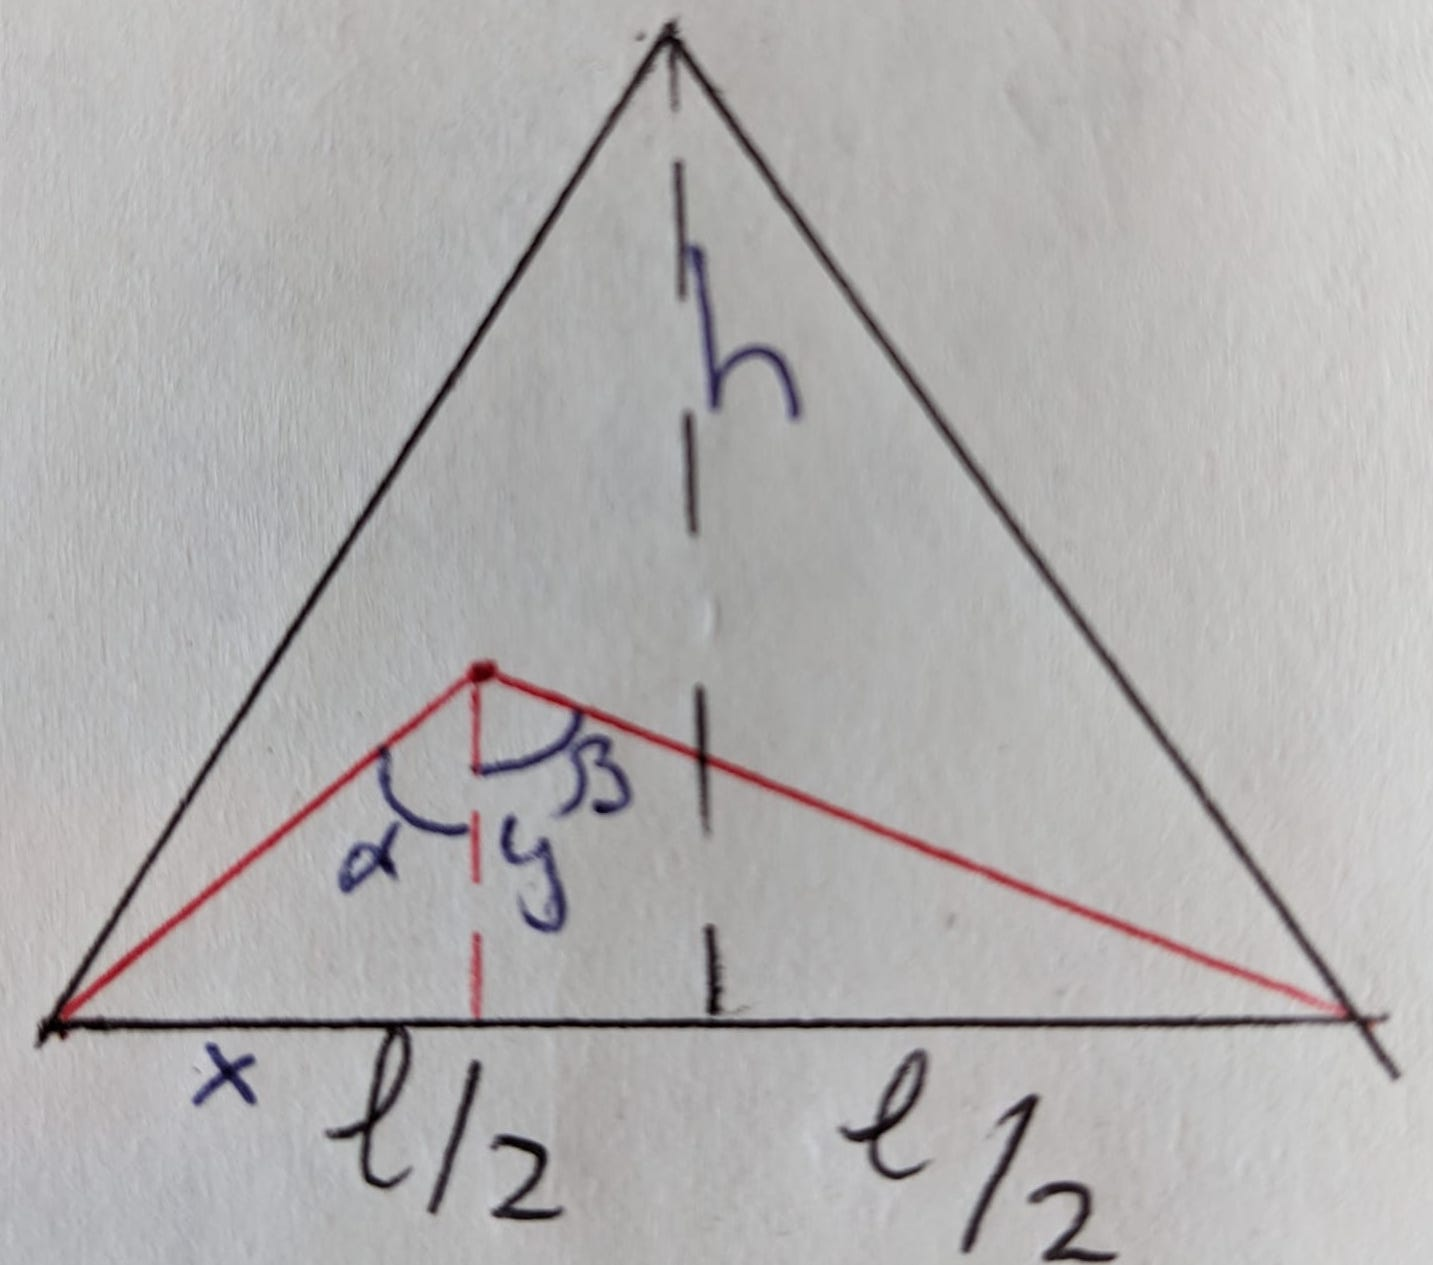
\includegraphics[width=\linewidth]{Figures/EquilateralTriangle.jpeg}
    \caption{Equilateral triangle}
    \label{fig:EquilateralTriangle}
\end{figure}

In this case, for any $x\in D$, we can caluculate the probability of hitting line $l_i$ as:
\begin{align*}
    \mathbb{P}\{ \text{hitting } l_i \ | \ X=x \} &= \frac{\alpha + \beta}{\pi} \\
    &= \left[ \arctan\left( \frac{x}{y} \right) + \arctan\left( \frac{l-x}{y}  \right) \right] / \pi \\
\end{align*}

Therefore, we get:
\begin{align}
    \mathbb{P}\{ \text{hitting } l_i \} &= \int_{0}^{l/2} \int_{0}^{x\cdot 2h/l} \left[ \arctan\left( \frac{x}{y} \right) + \arctan\left( \frac{l-x}{y}  \right) \right] / \pi \ dy dx
\end{align}


\subsection{General Rate equation}
Note that we have the recursive relation:
\begin{align}
    k_{i}(t) = k_{i}(t-1) + \mathbb{P}\{ \text{hitting } l_i \} \implies k_{i}(t) - k_{i}(t-1) = \mathbb{P}\{ \text{hitting } l_i \}.
\end{align}

Therefore, finding $\mathbb{P}\{ \text{hitting } l_i \}$ is key when we want to determine the rate equation.

\newpage
\newpage
\section{Square area calculation}
Let's say we can approximate the total adjacenct area as $k-1$ squares with combined lengths equal to segment length $L$, and average height equal to $H$. Then, we can calculate the probability of hitting the segment as:
\begin{itemize}

    \item \begin{align}
        \mathbb{P}\{ \text{hit} \ | \ x \in R(L,H) \} &= \int_{R(L,H)} \mathbb{P}\{ \text{hit} \ | \ (x,y) \in R(L,H) \} \ d\lambda
    \end{align}

    \item $R(L,H)$ is rectangle of dimensions $L \times H$.
    
    \item $\lambda \sim \text{Uniform}(R(l,H))$.
    
\end{itemize}

Note that:
\begin{align}
    \mathbb{P}\{ \text{hit} \ | \ (x,y) \in R(L,H) \} &= 2 \int_{0}^{H} \int_{0}^{L} \frac{ \alpha(x,y) }{ \pi }  \ dx dy \\
    &= \frac{2}{L H \pi} \int_{0}^{H} \int_{0}^{L} \arctan\left( \frac{x}{y} \right) \ dx dy 
\end{align}

We can calculate the integral as:
\begin{align}
    \int_{0}^{H} \int_{0}^{L} \arctan\left( \frac{x}{y} \right) \ dx dy &= \int_{0}^{H}\bigg[ x \arctan\left( \frac{x}{y} \right) - \frac{1}{2} y \log(x^2 + y^2) \bigg]_{x=0}^{x=L} \ dy \\
    &= \int_{0}^{H} \bigg[ L \arctan\left( \frac{L}{y} \right) - \frac{1}{2} y \log\left( \frac{L^2 + y^2}{y^2} \right) \bigg] \ dy \\
    &= L \bigg[ \frac{1}{2} L \log(L^2 + y^2) + y \arctan\left( \frac{L}{y} \right) \bigg]_{y=0}^{y=H} - \frac{1}{2} \bigg[ L^2 \log(y) + \frac{1}{2}(L^2 + y^2) \log\left( 1 + \frac{L^2}{y^2} \right) \bigg]_{y=0}^{y=H} \\
    &= \frac{L^2}{2} \log\left( 1 + \frac{H^2}{L^2} \right) + H L \arctan\left( \frac{L}{H} \right) - \frac{L^2}{2} \log(H) \frac{1}{4}(L^2 + H^2) \log\left( 1 + \frac{L^2}{H^2} \right) + \frac{L^2}{4} \bigg[ 2 \log(y) + \log\left( 1 + \frac{L^2}{y^2} \right) \bigg]_{y \to 0^{+}}.
\end{align}
Combining every























\end{document}
